\documentclass[a4paper]{article}  

\usepackage{mathtools}
\usepackage{amsthm}
\usepackage{amssymb}
\usepackage{tikz}
\usepackage{algpseudocode}

\title{CS270 Homework 4}
\author{Valkyrie Savage \thanks{Shiry, Mitar, Orianna, Daniel, Peggy, Ken, Andrew, Jaimie, Jan Vondr\'{a}k of Stanford, S\'{e}bastien Lahaie of Columbia, stat.ethz.ch, Wikipedia}}

\begin{document}
\maketitle

\begin{enumerate}

\item Maximum weight bipartite matching
	\begin{enumerate}
		\item For example:\\
		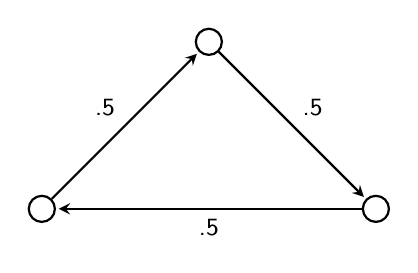
\begin{tikzpicture}[->,>=stealth,shorten >=1pt,auto,node distance=3cm,
 		thick,main node/.style={circle,fill=white!20,draw,font=\sffamily\Large\bfseries}]

  		\node[main node] (B) {};
  		\node[main node] (A) [below left of=B] {};
  		\node[main node] (C) [below right of=B] {};

  		\path[every node/.style={font=\sffamily\small}]
    		(A) edge node {.5} (B)
        		(B) edge node {.5} (C)
        		(C) edge node {.5} (A);
		\end{tikzpicture}
		\item 
			\begin{align}
				\max \sum_e{w_e x_e}\\
				\forall v \in V : \sum_{e=(u,v)} {x_e} &\leq 1 \\
				 \forall S \subseteq V s.t. \left| {S} \right| odd :
					\sum_{C(S, \overline{S})}{x_e} & \geq 1 \\
				x_e &\geq 0
			\end{align}
		\item We get the dual of the linear program by creating one dual variable per constraint.  For the first constraint, we note that we are adding each edge twice, once when it appears for the endpoint $u$ and once when it appears for the endpoint $v$, so we have $y_u,y_v$.  In the second constraint, we have $\tilde{y_S}$, which appears once each time an edge falls across a cut (defined by the set $cutsacross(e)$).  Our dual objective function minimizes across all the vertices we see and all the oddcut sets.  The result is this :
			\begin{align}
				\min \sum_{v \in V}{y_v} - \sum_{S \in oddcuts}{\tilde{y_S}} \\
				\forall e = (u,v) \in E :: w_e \leq y_v + y_u - \sum_{S \in cutsacross(e)}{\tilde{y_S}}
			\end{align}
	\end{enumerate}
	We notice that the dual has a variable $y_v$ for every vertex in the graph and a variable $\tilde{y_S}$ for every edge that falls across a cut.  The total cost of the solution is the sum of these two variables.  We can interpret the $y_v$s as the prices of the vertices and $w_e$ is the weight of the edge.  We see that $\tilde{y_S}$ is similar to a slack variable in that it is our wiggle room between the weight of an edge and the prices of its endpoints: but this slack variable is being ``charged'' to the subset that we are considering rather than to the prices of the vertices in order to create tight edges going across the gaps between odd subsets.
\item Convex bodies
	\begin{enumerate}
		\item We have two bodies, $A$ and $B$.  We select a point $a \in A$ where $a$ is the closest point in $A$ to $B$ and a point $b \in B$ where $b$ is the closest point in $B$ to $A$.  We construct a hyperplane between $a$ and $b$.  If the hyperplane intersects $A$ at a point $a_1$, then we know that $a$ was not, in fact, the closest point in $A$ to $B$.  Similarly, if the hyperplane intersects $B$ at a point $b_1$, then we know that $b$ was not, in fact, the closest point in $B$ to $A$, because since B is a convex set there will be a line of points $b_i \in B$ between $b$ and $b_1$, implying that there is some closer point in $B$ to $A$.
		\item Farkas B states that there is a solution for exactly one of
			\begin{enumerate}
				\item $Ax \leq b$
				\item $y^TA=0, y^Tb<0, y \geq 0$
			\end{enumerate}
			Both of these cannot be true, for the following reason:
			\begin{align}
				Ax &\leq b \\
				y^TAx &\leq y^Tb \\
				0 = y^TAx &\leq y^Tb <0 \\
				0 &< 0
			\end{align}
			One of them must be true, because if we assume that ii is not true, then i is true.  For ii to not be true, either $y^TA < 0$ or $y^TA > 0$.  If $y^TA < 0$, we can construct some $b, y$ s.t. $y^TA \leq y^Tb$:
			\begin{align}
				y^TA &\leq y^Tb \\
				A &\leq b
			\end{align}
			So we can construct some $x$ s.t. $Ax \leq b$ (for example the identity). \\
			If $y^TA > 0$:
			\begin{align}
				y^TA &> 0 > y^Tb \\
				A &> b
			\end{align}
			Given this, we can construct some $x$ ( $< 0$ ) s.t. $Ax \leq b$.
	\end{enumerate}

\item Facility Location
	\begin{enumerate}
		\item If we open all the facilities which are not yet open in our solution but which are open in the optimal solution, we would improve our connection cost by $C' - C$.  If we now consider this value averaged over all the facilities in the optimal solution, the average per unit facility cost is $\frac{C' - C}{F}$.  Our facility improves $C'$ by $\Delta$ and costs $f$.  It is possible to, and we do, select our facility such that these improvements are better than or equal to the average (law of averages!), i.e.$\Delta \geq \frac{f(C' - C)}{F} \implies \frac{\Delta}{f} \geq \frac{C' - C}{F}$.
		\item We begin with the result of the problem above, which gives us the cost and benefit ratio of a ``good'' facility.
			\begin{align}
				\frac{\Delta_i}{f_i} &\geq \frac{C' - C}{F} \\
				f_i &\leq \frac{\Delta_i F}{C' - C} \\
				facility-total = f_i - \Delta_i &\leq \frac{\Delta_i F}{C' - C} - \Delta_i
			\end{align}
			Now we want to integrate, since we can consider adding facilities to approach C from C'.  We want to do this in as large of steps as possible for as long as possible, but will eventually consider infinitesimally small steps.  We consider our integration bounds : we want to start at $F+C$ (the optimal) and go to what we currently have, which is $2F+3C$.
			\begin{align}
				\int_a^b{dC' \frac{F}{C' - C} - dC'} \\
				= \left. F\ln \frac{C' - C}{F} - C \right|_{F+C}^{2F+3C} \\
				= F \ln \frac{2F + 2C}{F} - (2F + 3C) - F \ln \frac{F}{F} + F + C+ 3F + 3C \\
				= F \ln \frac{2F + 2C}{F} + F + F + C \\
				= F + C plus (1+\ln\frac{2F + 2C}{F})
			\end{align}
			Which is the desired solution.
		\item consider the distances 1 or 3
	\end{enumerate}

\item Using the second moment calculation algorithms from class, we can get the following values:
	\begin{align}
		\sum{f_r(a)^2} \\	
		\sum{f_s(a)^2} \\
		\sum{(f_r(a)+f_s(a))^2}	
	\end{align}
	We observe that this last one is subject to the binomial theorem:
	\begin{align}
		\sum{f_r(a)^2 + 2f_r(a)f_s(a) + f_s(a)^2}
	\end{align}
	From this we can subtract the other two second moments we calculated and divide our result by 2, leaving us with our desired solution
	\begin{align}
		\sum{f_r(a)f_s(a)}
	\end{align}
	The error bound that we see for this is based on the errors of all the terms we put into its calculation:
	\begin{align}
		\frac{1}{2}((f_r(a)^2 + 2f_r(a)f_s(a) + f_s(a)^2)(1 \pm \epsilon) - f_r(a)^2(1 \pm \epsilon) - f_s(a)^2(1 \pm \epsilon)) \\
		= f_r(a)f_s(a) \pm \epsilon( f_r(a)f_s(a) + f_r(a)^2 + f_s(a)^2 )
	\end{align}
\item Project description \\
	Working with Mitar to analyze/illustrate multi-way voting algorithms.
\end{enumerate}
\end{document}